\section{M3 extension: an explicit Markov movie network}
\subsection{What changed, and why it might help}
The M2 latent-trait model already is probabilistic. Its independent movie priors,
however, do not explicitly connect similar movies. M3 adds a separate Gaussian
Markov random field (GMRF) prior to a matrix-factorization model. An undirected
edge encourages two movies' latent vectors to remain similar. This can reduce
estimation variance when ratings are sparse or unreliable, but a misleading or
overly strong edge can introduce bias. Improvement is a hypothesis to test,
not a property guaranteed by the word ``Markov.''

The new model uses maximum a posteriori (MAP) estimation by alternating block
minimization. It does not add graph messages to the original EP implementation.
Consequently, comparing GMRF-MAP with EP changes both the prior and the fitting
method/likelihood. The controlled graph ablation is \textbf{GMRF-MAP versus
MF-MAP with $\gamma=0$}, sharing the data, initialization, regularization,
training budget and validation rules.

\subsection{Building the graph from available evidence}
\label{sec:graphconstruction}
For each split, the graph is constructed from training ratings and fixed movie
genres only. Five alternating regularized bias updates estimate $\mu,b_u,b_i$;
their residuals are $e_{ui}=R_{ui}-\mu-b_u-b_i$. Each movie's sparse residual
column is normalized. Positive residual cosine similarities are multiplied by
$n_{ij}/(n_{ij}+20)$, where $n_{ij}$ is the number of common training users;
similarities based on fewer than five common users are set to zero.

Genres are represented by an 18-dimensional multi-hot vector, normalized to
unit length before computing genre cosine similarity. Default affinities mix
90\% residual similarity and 10\% genre similarity. Each movie retains its top
20 positive neighbours; ties use mapped movie IDs. The union is symmetrized
using the maximum of the two directed weights, so final degrees can exceed 20.
If $A$ denotes this symmetric affinity, $W=D_A^{-1/2}AD_A^{-1/2}$.
We then recompute $D_{ii}=\sum_jW_{ij}$ and set $L=D-W$.
The diagonal of $W$ is zero. This is a deterministic similarity construction,
not causal discovery or recovery of a known true graph. Across the five main
splits, the graph has 56,408--56,575 undirected movie edges (mean 56,508),
mean degree 30.50, density 0.823\%, and no isolated movie nodes. These are
representation statistics, not edge-recovery accuracy. Because $W$ is
estimated from training ratings, this is a data-dependent, empirical-Bayes-style
regularization construction. We condition on the resulting $W$ and do not
propagate uncertainty about its edges.

\begin{figure}[!htbp]\centering
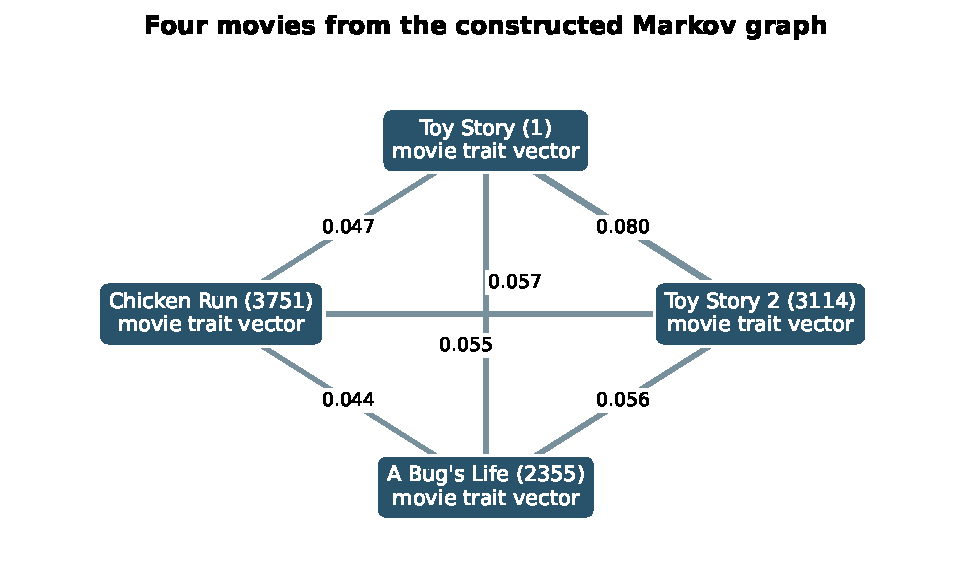
\includegraphics[width=.92\linewidth]{../../Results/analysis/plots/movie_subgraph.pdf}
\caption{Actual seed-42 subgraph: Toy Story and its three strongest neighbours.
Node labels give titles and raw MovieLens IDs; displayed edge labels are the
normalized weights. Each node represents a movie's latent vector; each edge
induces the pairwise factor in Equation~\ref{eq:gmrfprior}. The full graph has
many other neighbours. Similarity is not a causal claim.}
\end{figure}

\subsection{Factors, conditional independence and MAP objective}
With $Q_i\in\mathbb R^K$ for movie $i$, the movie prior is
\begin{align}
p(Q\mid W)&\propto
 \prod_i \exp\!\left(-\frac{\lambda}{2}\|Q_i\|^2\right)
 \prod_{\{i,j\}\in E}\exp\!\left(-\frac{\gamma w_{ij}}{2}\|Q_i-Q_j\|^2\right),\label{eq:gmrfprior}\\
J&=\lambda I+\gamma L,\qquad
\operatorname{tr}(Q^TLQ)=\sum_{\{i,j\}\in E}w_{ij}\|Q_i-Q_j\|^2.
\end{align}
Each trait coordinate across movies has Gaussian precision $J$.
For any nonzero $x$, $x^TJx=\lambda\|x\|^2+
\gamma\sum_{\{i,j\}\in E}w_{ij}(x_i-x_j)^2>0$ when $\lambda>0$.
Thus the prior is proper, including for disconnected graphs. A zero off-diagonal
entry in $J$ expresses conditional independence in this prior, given all other
movie variables. It does not imply marginal independence or the absence of
posterior dependence after observing ratings.

The conditional for one coordinate of movie $i$ is
\begin{equation}
 Q_{ik}\mid Q_{-i,k},W\sim\N\!\left(
 \frac{\gamma\sum_jw_{ij}Q_{jk}}{\lambda+\gamma D_{ii}},
 \frac{1}{\lambda+\gamma D_{ii}}\right).
\end{equation}
This gives a precise meaning to ``neighbours share information.'' Nodes are
latent variables, and edges encode pairwise probability factors; they are not
causal arrows, a neural network, or time transitions in a Markov chain.

Using $f_{ui}=\mu+b_u+b_i+P_u^TQ_i$, independent Gaussian user priors, bias
priors and unit-variance Gaussian numeric-rating likelihood gives the energy
\begin{equation}
\begin{split}
\mathcal E={}&\frac12\sum_{(u,i)\in\mathcal D}(R_{ui}-f_{ui})^2
+\frac\lambda2(\|P\|_F^2+\|Q\|_F^2)\\
&+\frac{\lambda_b}{2}(\|b_U\|^2+\|b_I\|^2)
+\frac\gamma2\operatorname{tr}(Q^TLQ).
\end{split}\label{eq:energy}
\end{equation}
Defaults are $K=8$ and $\lambda=\lambda_b=10$. Holding other blocks fixed,
each user/movie vector and its bias solve a $(K+1)$-dimensional linear system.
For a movie, the trait block gains $\gamma D_{ii}I$ on the left and
$\gamma\sum_jw_{ij}Q_j$ on the right. Sequential movie updates use the newest
neighbours (Gauss--Seidel). Each exact block update cannot increase this energy;
joint bilinear optimization remains nonconvex, so this is not a global-optimum
guarantee. Source: \code{gmrf.py}, functions \code{graph}, \code{als} and
\code{objective}.

\subsection{Prediction and the meaning of uncertainty}
MAP stores point estimates of the traits and biases. A single Gaussian
observation variance is fitted on validation NLL and integrated between the
same five rating intervals as EP. This produces probabilities and an expected
star rating for common KPI evaluation. The separately reported clipped score
$\min(5,\max(1,f_{ui}))$ is another point decoder. The MAP probability wrapper
represents residual variation; it is \textbf{not a full Bayesian posterior}
over the fitted parameters. EP retains approximate parameter uncertainty but
uses a factorized posterior and additional score-Gaussian approximation.

For $T$ epochs, dense small-block solves cost
$O(T[N(K+1)^2+(U+I)(K+1)^3+|E|K])$. The sparse graph requires $O(|E|)$
storage. Graph construction evaluates movie similarities in row blocks and can
be costly for a large catalogue; batching reduces peak dense memory, not its
pairwise nature. Graph building and hyperparameter search are reported in
addition to fitting the selected candidate.
